% !TeX program = xelatex
% Author: Huihuo Zheng, huihuo.zheng@anl.gov
% Copyright: Trinity Science 2026
%
% Hands-On: Agentic AI for AmSC --- the workshop deck for this tutorial.
% Audience: scientists and facility staff doing the labs (hands-on).
%
% Build:  make handson      (or: xelatex amsc_agentic_ai_handson.tex, twice)
% Needs:  xelatex, metropolis, fontawesome5, tcolorbox, listings.
%         No -shell-escape, no Pygments: code is set with `listings`, not minted.
%
% ---------------------------------------------------------------------------
% Structure borrowed from the Service-Enabled Science 2026 Session 05 deck
% (ses_agentic_workflows.tex) --- its arc of
%     from services to agents -> building blocks -> hands-on -> where this goes
% carries over, rescoped from ALCF-only to this tutorial's three facilities and
% MAG. The SES deck's sesalcf theme and sesalcf-assets/ are deliberately NOT
% vendored here: that theme is an unlicensed third-party fork and its assets are
% official DOE/Argonne marks, which this public repository should not
% redistribute. This deck therefore reuses the preamble style already in
% amsc_agentic_ai.tex instead.
%
% SELF-CONTAINED BY DESIGN. Every figure is TikZ; the only external file is an
% optional logo, guarded by \IfFileExists. Do not add an \includegraphics of an
% asset outside slides/, and do not point \graphicspath outside this directory
% --- the sibling deck amsc_agentic_ai.tex does both and consequently cannot be
% built from a fresh clone of this repository.
%
% Design intent (see .claude/skills/beamer-slides/SKILL.md):
%   - One signature element per slide; everything else stays quiet.
%   - Informative titles: the title states the takeaway, not the topic.
%   - Figures over prose. Boxes only where something is separated from
%     something else; otherwise \sechead and \takeaway.
%   - Colour is semantic and fixed deck-wide:
%       accentteal  the agent / MCP layer -- what this tutorial adds
%       labnavy     facilities, schedulers, and human authority
%       accentgold  models and MAG
%       midgray     the manual status quo, and muted asides
% ---------------------------------------------------------------------------
\documentclass[aspectratio=169,11pt]{beamer}

\usetheme{metropolis}
\usepackage{fontspec}
\usepackage{graphicx}
\usepackage{tikz}
\usetikzlibrary{arrows.meta,positioning,shapes.geometric,fit,calc}
\usepackage{tcolorbox}
\tcbuselibrary{skins,breakable}
\usepackage{fontawesome5}
\usepackage{booktabs}
\usepackage{array}
\usepackage{listings}

% ---------------------------------------------------------------- palette
\definecolor{labnavy}{RGB}{18,42,73}
\definecolor{labink}{RGB}{40,44,52}
\definecolor{accentgold}{RGB}{223,161,54}
\definecolor{accentteal}{RGB}{0,137,123}
\definecolor{accentblue}{RGB}{41,98,168}
\definecolor{lightgray}{RGB}{245,246,248}
\definecolor{midgray}{RGB}{110,118,129}
\definecolor{okgreen}{RGB}{35,140,80}

\setbeamercolor{background canvas}{bg=white}
\setbeamercolor{palette primary}{bg=labnavy,fg=white}
\setbeamercolor{frametitle}{bg=labnavy,fg=white}
\setbeamercolor{progress bar}{fg=accentteal,bg=lightgray}
\setbeamercolor{normal text}{fg=labink}
\setbeamercolor{alerted text}{fg=accentgold}
\setbeamercolor{footline}{fg=midgray}
\setbeamerfont{footline}{size=\tiny}
\setlength{\leftmargini}{14pt}

% Safe zones: explicit L/R margin, plus a reserved strip above the page number.
\setbeamersize{text margin left=9mm, text margin right=9mm}
\addtobeamertemplate{footline}{\vspace*{2mm}}{}

% ---------------------------------------------------------------- metadata
\newcommand{\deckauthor}{Huihuo Zheng}
\newcommand{\deckemail}{huihuo.zheng@anl.gov}
\newcommand{\deckinstitute}{Argonne Leadership Computing Facility (ALCF)}
\title{Hands-On: Agentic AI for AmSC}
\date{October 2026}

% ---------------------------------------------------------------- logo
% logos/trinity_logo.pdf is in this repository, so this resolves by default.
% An argonne_logo.pdf dropped in alongside it takes precedence; if neither is
% present the deck still builds, falling back to a text lockup rather than a
% fabricated institutional mark.
\newcommand{\decklogo}[1][0.16\textwidth]{%
  \IfFileExists{logos/argonne_logo.pdf}%
    {\includegraphics[width=#1]{logos/argonne_logo.pdf}}%
    {\IfFileExists{logos/trinity_logo.pdf}%
      {
\includegraphics[width=#1]{logos/trinity_logo.pdf}}%
      {\textbf{\textsc{\textcolor{labnavy}{Argonne National Laboratory}}}}}}

% ---------------------------------------------------------------- boxes
\newtcolorbox{featbox}[2]{
  enhanced,
  colback=lightgray, colframe=#1, boxrule=0.6pt, arc=3pt,
  left=6pt, right=6pt, top=4pt, bottom=4pt,
  % title is BRACED: an unbraced #2 lets a comma in the title text be parsed
  % as a pgfkeys separator ("... run, delegated" -> unknown key /tcb/delegated).
  title={#2}, colbacktitle=#1, coltitle=white,
  fonttitle=\bfseries\small, boxsep=1pt,
  halign title=flush left,
  drop fuzzy shadow
}
\newtcolorbox{chatbubble}[2]{
  enhanced,
  colback=#1!12, colframe=#1!60!black, boxrule=0.5pt, arc=5pt,
  left=8pt, right=8pt, top=3pt, bottom=3pt, width=\linewidth,
  title={#2}, colbacktitle=#1!60!black, coltitle=white,
  fonttitle=\bfseries\footnotesize, boxsep=1pt,
  drop fuzzy shadow
}

% De-boxing tools: a coloured header + rule instead of a card, and a bold
% lead-in instead of a trailing callout box.
\newcommand{\sechead}[2]{{\small\color{#1}\bfseries #2}\par\vspace{1.5pt}%
  {\color{#1!45}\rule{\linewidth}{0.6pt}}\par\vspace{4pt}}
\newcommand{\takeaway}[3][labnavy]{{\color{#1}\bfseries #2} #3}

% A small caption tag above a code block.
\newcommand{\codetag}[2][labnavy]{%
  \par\vspace{1pt}{\scriptsize\color{#1}\bfseries #2}\par\vspace{1pt}}

% ---------------------------------------------------------------- code styles
\lstdefinestyle{shell}{
  language=bash,
  basicstyle=\ttfamily\scriptsize\color{labink},
  keywordstyle=\color{accentblue}\bfseries,
  commentstyle=\color{midgray}\itshape,
  stringstyle=\color{accentteal},
  backgroundcolor=\color{lightgray},
  frame=single, framerule=0.4pt, rulecolor=\color{midgray!60},
  breaklines=true, columns=fullflexible,
  xleftmargin=4pt, xrightmargin=4pt, framexleftmargin=4pt,
  showstringspaces=false, numbers=none, aboveskip=2pt, belowskip=2pt
}
\lstdefinestyle{pysnip}{
  language=Python,
  basicstyle=\ttfamily\scriptsize\color{labink},
  keywordstyle=\color{accentblue}\bfseries,
  commentstyle=\color{midgray}\itshape,
  stringstyle=\color{accentteal},
  backgroundcolor=\color{lightgray},
  frame=single, framerule=0.4pt, rulecolor=\color{midgray!60},
  breaklines=true, columns=fullflexible,
  xleftmargin=4pt, xrightmargin=4pt, framexleftmargin=4pt,
  showstringspaces=false, numbers=none, aboveskip=2pt, belowskip=2pt
}
\lstdefinestyle{plainsnip}{
  basicstyle=\ttfamily\scriptsize\color{labink},
  backgroundcolor=\color{lightgray},
  frame=single, framerule=0.4pt, rulecolor=\color{midgray!60},
  breaklines=false, columns=fullflexible,
  xleftmargin=4pt, xrightmargin=4pt, framexleftmargin=4pt,
  showstringspaces=false, numbers=none, aboveskip=2pt, belowskip=2pt
}

% ---------------------------------------------------------------- graphics
% Deliberately local-only. See the header note.
\graphicspath{{}{logos/}}

% ---------------------------------------------------------------- TikZ styles
\tikzset{
  toolnode/.style={rounded corners=4pt, draw=#1, line width=1pt,
    fill=#1!10, inner sep=5pt, align=center, font=\scriptsize},
  facilitynode/.style={rounded corners=3pt, draw=labnavy, line width=0.8pt,
    fill=labnavy!8, inner sep=4pt, align=center, font=\scriptsize},
  agentnode/.style={rounded corners=4pt, draw=labnavy, line width=1.2pt,
    fill=labnavy!10, inner sep=6pt, align=center, font=\small\bfseries},
  partnode/.style={rounded corners=4pt, draw=#1, line width=1pt,
    fill=#1!8, inner sep=5pt, align=center, font=\scriptsize},
  flow/.style={-{Stealth[length=2.2mm]}, line width=0.85pt, draw=#1},
  tag/.style={rounded corners=2pt, fill=#1!15, draw=#1, line width=0.4pt,
    inner xsep=3pt, inner ysep=1.5pt, font=\tiny\bfseries, text=#1!70!black},
}

\begin{document}

% ================================================================ TITLE
{
\setbeamertemplate{logo}{}
\begin{frame}[plain]
  \begin{columns}[c]
    \begin{column}{0.30\textwidth}
      \centering
      \decklogo[0.88\textwidth]
    \end{column}
    \begin{column}{0.68\textwidth}
      {\usebeamerfont{title}\usebeamercolor[fg]{title}\Large\bfseries
        Hands-On: Agentic AI for AmSC\par}
      \vspace{5pt}
      {\normalsize\color{midgray}
        MAG \textperiodcentered\ MCP \textperiodcentered\ IRI
        \textperiodcentered\ Globus Compute\\
        from your laptop to three DOE facilities\par}
      \vspace{14pt}
      {\small
        \deckauthor\\
        \deckinstitute\\
        \insertdate}
    \end{column}
  \end{columns}
  \vfill
  {\footnotesize\color{midgray}\faEnvelope[regular]\ \deckemail
   \hfill\texttt{github.com/zhenghh04/amsc\_agentic\_ai}\par}
\end{frame}
}

% ================================================================================
\section{From services to agents}
% ================================================================================

% ---------------------------------------------------------------- THE SPINE
\begin{frame}{Three parts carry one workload from your laptop to three facilities}
  \centering
  \begin{tikzpicture}[line width=0.85pt]
    \node[partnode=accentteal, text width=3.1cm] (p1) at (0,0)
      {\faLaptop\ \textbf{Part 1 --- Laptop}\\[2pt]
       \tiny\normalfont 00 setup (MAG)\\[-1pt]\tiny 01 simulation\\[-1pt]
       \tiny 02 training\\[-1pt]\tiny 03 inference};
    \node[partnode=accentblue, text width=3.1cm, right=10mm of p1] (p2)
      {\faServer\ \textbf{Part 2 --- HPC}\\[2pt]
       \tiny\normalfont 05 run it natively\\[-1pt]\tiny on a login node\\[-1pt]
       \tiny (modules, scheduler)};
    \node[partnode=labnavy, text width=3.1cm, right=10mm of p2] (p3)
      {\faNetworkWired\ \textbf{Part 3 --- IRI}\\[2pt]
       \tiny\normalfont 07 MCP setup\\[-1pt]\tiny 08 job submission\\[-1pt]
       \tiny 09 remote functions};

    \draw[flow=midgray] (p1) -- (p2);
    \draw[flow=midgray] (p2) -- (p3);

    \node[below=7mm of p2, text width=11.6cm, align=center,
          rounded corners=3pt, fill=lightgray, draw=midgray!50,
          inner sep=4pt, font=\scriptsize] (spine)
      {\textbf{One spine, scaled three times:}\;
       simulation \textperiodcentered\ training \textperiodcentered\ inference};
    \draw[flow=midgray, dashed] (p1.south) -- (p1.south |- spine.north);
    \draw[flow=midgray, dashed] (p3.south) -- (p3.south |- spine.north);
  \end{tikzpicture}
  \par\vspace{7pt}
  \takeaway[accentteal]{The science never changes.}{%
    Only \emph{where} it runs and \emph{who} drives the mechanics.}
\end{frame}

% ---------------------------------------------------------------- PROBLEM
\begin{frame}{Scientists spend their first hours on mechanics, not on science}
  \begin{columns}[T,totalwidth=\textwidth]
    \begin{column}{0.47\textwidth}
      \begin{featbox}{midgray}{\faTerminal\ The manual loop today}
        \scriptsize
        \begin{enumerate}\setlength\itemsep{1pt}
          \item SSH to a login node
          \item Read module docs, hand-write a script
          \item Fix account, queue, walltime, paths
          \item Submit, then poll \texttt{qstat}
          \item Parse the error, edit, resubmit
          \item Move the output files by hand
        \end{enumerate}
      \end{featbox}
    \end{column}
    \begin{column}{0.06\textwidth}\end{column}
    \begin{column}{0.47\textwidth}
      \begin{featbox}{accentteal}{\faRobot\ The same run, delegated}
        \scriptsize
        \textit{``Run my training script on two Polaris nodes and tell me when
        it converges.''}
        \vspace{3pt}
        \begin{itemize}\setlength\itemsep{1pt}
          \item[\faCheckCircle] Resolves account, queue, paths
          \item[\faCheckCircle] Stages the script and submits
          \item[\faCheckCircle] Monitors; diagnoses failures
          \item[\faCheckCircle] Reports back with evidence
        \end{itemize}
      \end{featbox}
    \end{column}
  \end{columns}
  \vspace{6pt}
  \takeaway{The mechanics are the bottleneck}{%
    --- and every one of them is already an API. This tutorial wires an agent
    to those APIs.}
\end{frame}

% ---------------------------------------------------------------- AGENT LOOP
\begin{frame}{An agent is a loop: a model, some tools, a stopping condition}
  \centering
  \begin{tikzpicture}[line width=0.85pt]
    \node[agentnode, text width=2.2cm] (model) at (0,0)
      {\faBrain\ \textbf{Model}\\[2pt]\tiny\normalfont MAG};
    \node[toolnode=accentteal, text width=2.2cm] (decide) at (3.3,0)
      {\faSitemap\ \textbf{Decide}\\[1pt]\tiny\normalfont call a tool,\\[-1pt]
       \tiny or answer?};
    \node[toolnode=labnavy, text width=2.2cm] (act) at (6.6,0)
      {\faBolt\ \textbf{Act}\\[1pt]\tiny\normalfont run it,\\[-1pt]
       \tiny capture the result};
    \node[toolnode=midgray, text width=2.2cm] (obs) at (9.9,0)
      {\faEye\ \textbf{Observe}\\[1pt]\tiny\normalfont append it\\[-1pt]
       \tiny to the context};

    \draw[flow=midgray] (model) -- (decide);
    \draw[flow=midgray] (decide) -- (act);
    \draw[flow=midgray] (act) -- (obs);
    \draw[flow=midgray] (obs.south) -- ++(0,-0.75)
      -| node[pos=0.25,below,font=\tiny\itshape,text=midgray]
      {repeat until done} (model.south);
  \end{tikzpicture}
  \par\vspace{10pt}
  \begin{columns}[T,totalwidth=\textwidth]
    \begin{column}{0.47\textwidth}
      \sechead{labnavy}{\faCode\ You can read the whole thing}
      \scriptsize Bonus page B builds this loop against MAG in about twenty
      lines. Claude Code and opencode are this loop, hardened.
    \end{column}
    \begin{column}{0.06\textwidth}\end{column}
    \begin{column}{0.47\textwidth}
      \sechead{accentteal}{\faWrench\ The loop is the easy part}
      \scriptsize The value is in \emph{which} tools the model can reach ---
      and whether they are safe to hand it.
    \end{column}
  \end{columns}
\end{frame}

% ---------------------------------------------------------------- MCP
\begin{frame}{MCP is how the agent reaches a facility by name, not by URL}
  \begin{columns}[c, totalwidth=\textwidth]
    \begin{column}{0.44\textwidth}
      \centering
      \begin{tikzpicture}[line width=0.85pt]
        % Vertical gaps are sized so the \tiny arrow labels sit in clear space:
        % at 1.6cm pitch the labels collided with the box edges above and below.
        \node[agentnode, text width=2.9cm] (agent) at (0,3.8)
          {\faRobot\ \textbf{Agent}\\[1pt]
           \tiny\normalfont Claude Code / opencode};
        \node[toolnode=accentteal, text width=2.9cm] (mcp) at (0,1.9)
          {\faPlug\ \textbf{MCP server}\\[1pt]\tiny\normalfont named tools\\[-1pt]
           \tiny + JSON schemas};
        \node[toolnode=labnavy, text width=2.9cm] (svc) at (0,0)
          {\faServer\ \textbf{Facility services}\\[1pt]
           \tiny\normalfont IRI, Globus, docs};

        % Arrows sit inboard of x=+-0.55 so a label hung off their outer side
        % still lands inside the 2.9cm box width above and below it.
        \draw[flow=accentteal] ($(agent.south)+(-0.55,0)$)
          -- node[left,font=\tiny,text=midgray,inner sep=2pt]{list}
          ($(mcp.north)+(-0.55,0)$);
        \draw[flow=accentteal] ($(mcp.north)+(0.55,0)$)
          -- node[right,font=\tiny,text=midgray,inner sep=2pt]{call}
          ($(agent.south)+(0.55,0)$);
        \draw[flow=labnavy] ($(mcp.south)+(-0.3,0)$)
          -- node[right,font=\tiny,text=midgray,inner sep=3pt]{HTTPS + token}
          ($(svc.north)+(-0.3,0)$);
      \end{tikzpicture}
    \end{column}
    \begin{column}{0.04\textwidth}\end{column}
    \begin{column}{0.50\textwidth}
      \sechead{labnavy}{\faQuestionCircle\ What MCP buys you}
      \scriptsize
      \begin{itemize}\setlength\itemsep{2.5pt}
        \item[\faSearch] \textbf{Discovered.} The agent asks the server what it
          can do --- no endpoints, no hand-built payloads.
        \item[\faCheckCircle] \textbf{Typed.} One schema per tool, so bad
          arguments fail \emph{before} a job runs.
        \item[\faUserShield] \textbf{Scoped by you.} The server holds the
          token and decides what is reachable.
        \item[\faWrench] \textbf{Configured once.} \texttt{.mcp.json} for
          Claude Code, \texttt{opencode.jsonc} for opencode.
      \end{itemize}
    \end{column}
  \end{columns}
\end{frame}

% ================================================================================
\section{Building blocks}
% ================================================================================

% ---------------------------------------------------------------- THE FIVE SERVERS
\begin{frame}{Five MCP servers give the agent knowledge, reach, and data movement}
  \centering
  \begin{tikzpicture}[line width=0.85pt]
    % The tool column is CHAINED (below=4mm of <prev>), not positioned by
    % offset from `agent'. An `above right=-1mm of agent' offset is measured
    % from the anchor, so the gap it leaves depends on each box's own height:
    % the earlier version put MAG/knowledge and IRI/globus-compute flush
    % against each other.
    \node[toolnode=accentgold, text width=2.6cm] (mag) at (0,0)
      {\faComments\ \textbf{MAG}\\[1pt]\tiny\normalfont the model itself};
    \node[toolnode=accentteal, text width=2.6cm, below=3mm of mag] (know)
      {\faBookOpen\ \textbf{knowledge}\\[1pt]\tiny\normalfont live facility docs};
    \node[toolnode=accentteal, text width=2.6cm, below=3mm of know] (iri)
      {\faPlug\ \textbf{3 $\times$ IRI}\\[1pt]\tiny\normalfont alcf / nersc / olcf};
    \node[toolnode=accentteal, text width=2.6cm, below=3mm of iri] (gc)
      {\faGlobe\ \textbf{globus-compute}\\[1pt]\tiny\normalfont functions on MEPs};

    \node[agentnode, text width=2.0cm] (agent)
      at ($(mag.west)!0.5!(gc.west)-(2.5,0)$)
      {\faBrain\ \textbf{Agent}\\[1pt]\tiny\normalfont your laptop};

    \node[facilitynode, text width=1.7cm] (f1)
      at ($(know.east)!0.5!(iri.east)+(2.1,0)$)
      {\textbf{Polaris}\\[-1pt]\tiny ALCF};
    \node[facilitynode, text width=1.7cm, above=3mm of f1] (f0)
      {\textbf{Perlmutter}\\[-1pt]\tiny NERSC};
    \node[facilitynode, text width=1.7cm, below=3mm of f1] (f2)
      {\textbf{Frontier}\\[-1pt]\tiny OLCF};

    \draw[flow=accentgold] (agent.east) to[bend left=16] (mag.west);
    \draw[flow=accentteal] (agent.east) to[bend left=5] (know.west);
    \draw[flow=accentteal] (agent.east) to[bend right=5] (iri.west);
    \draw[flow=accentteal] (agent.east) to[bend right=16] (gc.west);

    \draw[flow=labnavy, dashed] (iri.east) -- (f1.west);
    \draw[flow=labnavy, dashed] (iri.east) to[bend left=10] (f0.west);
    \draw[flow=labnavy, dashed] (iri.east) to[bend right=10] (f2.west);
    \draw[flow=midgray, dashed] (gc.east) to[bend right=12] (f1.south west);
  \end{tikzpicture}
  \par\vspace{3pt}
  \small
  \takeaway[accentteal]{Knowledge, reach, data --- and judgment.}{%
    The fourth leg is the \texttt{submit-job} skill.}
\end{frame}

% ---------------------------------------------------------------- AGENT CORE
\begin{frame}[fragile]{Agent core: three variables point your agent at MAG}
  \begin{columns}[T,totalwidth=\textwidth]
    \begin{column}{0.56\textwidth}
      \codetag{\faTerminal\ Claude Code --- Anthropic wire}
\begin{lstlisting}[style=shell]
export ANTHROPIC_BASE_URL=\
https://i2-api.genesis.american-science-cloud.org
export ANTHROPIC_AUTH_TOKEN=$AMSC_I2_API_KEY
export ANTHROPIC_MODEL=claude-sonnet-4-6
claude
\end{lstlisting}
      \codetag[accentteal]{\faRobot\ opencode --- OpenAI wire, note the /v1}
\begin{lstlisting}[style=shell]
# opencode.jsonc already sets:
#   baseURL .../american-science-cloud.org/v1
read -rs AMSC_I2_API_KEY; export AMSC_I2_API_KEY
opencode
\end{lstlisting}
    \end{column}
    \begin{column}{0.02\textwidth}\end{column}
    \begin{column}{0.42\textwidth}
      \sechead{labnavy}{\faInfoCircle\ Why two wires}
      \scriptsize
      \begin{itemize}\setlength\itemsep{2.5pt}
        \item[\faKey] MAG is a \textbf{public-cloud} gateway. Your PAT is the
          only credential --- no VPN.
        \item[\faExclamationTriangle] MAG speaks \textbf{both} wires. opencode
          needs the OpenAI one \emph{with} \texttt{/v1}; the Anthropic wire
          answers with a 302 it will not follow.
        \item[\faUserShield] Never paste the PAT on a command line ---
          \texttt{read -rs} keeps it out of shell history.
      \end{itemize}
    \end{column}
  \end{columns}
\end{frame}

% ---------------------------------------------------------------- IRI
\begin{frame}[fragile]{One tool shape, three facilities behind it}
  \begin{columns}[T,totalwidth=\textwidth]
    \begin{column}{0.52\textwidth}
      \codetag{\faPlug\ the same call, a different server}
\begin{lstlisting}[style=pysnip]
submit_job(
    system="polaris",
    script_path="run.sh",
    queue="debug",
    nodes=2, walltime="00:10:00",
)
get_job_status(job_id="...")
read_file(path=".../job.out", tail=40)
\end{lstlisting}
      {\scriptsize\color{midgray}\faInfoCircle\ The agent picks the server from
       the system you name --- you do not.}
    \end{column}
    \begin{column}{0.03\textwidth}\end{column}
    \begin{column}{0.45\textwidth}
      \sechead{labnavy}{\faNetworkWired\ What each server fronts}
      \scriptsize
      \begin{tabular}{@{}ll@{}}
        \toprule
        \textbf{Server} & \textbf{Scheduler} \\
        \midrule
        \texttt{alcf-iri}  & PBS (Polaris, Aurora) \\
        \texttt{nersc-iri} & Slurm (Perlmutter) \\
        \texttt{olcf-iri}  & Slurm (Frontier) \\
        \bottomrule
      \end{tabular}
      \par\vspace{6pt}
      \takeaway[accentteal]{One login each.}{%
        Tokens are short-lived, OAuth2, and yours --- the server holds them,
        the model never sees them.}
    \end{column}
  \end{columns}
\end{frame}

% ---------------------------------------------------------------- GLOBUS COMPUTE
\begin{frame}[fragile]{Globus Compute runs your function where the data already is}
  \begin{columns}[T,totalwidth=\textwidth]
    \begin{column}{0.52\textwidth}
      \codetag{\faGlobe\ Lab 09 --- no endpoint to babysit}
\begin{lstlisting}[style=pysnip]
register_function(source=\
    "def f(n):\n    return n * 2")
run_function(function_id="...", args=[21])
get_result(task_id="...")        # -> 42
\end{lstlisting}
      {\scriptsize\color{midgray}A \textbf{Multi-User Endpoint} is already
       running at the facility. You submit a function, not a job script.}
    \end{column}
    \begin{column}{0.03\textwidth}\end{column}
    \begin{column}{0.45\textwidth}
      \sechead{accentgold}{\faExclamationTriangle\ Two lessons worth the slide}
      \scriptsize
      \begin{itemize}\setlength\itemsep{3pt}
        \item[\faCode] \textbf{Serialize by source.} The endpoint's Python is
          not yours; shipping \emph{source} rather than a pickle is what makes
          a version mismatch survivable.
        \item[\faDatabase] \textbf{Filesystems are opt-in.} A MEP sees only the
          mounts it was configured with --- and Polaris cannot see Aurora's
          \texttt{/flare} at all.
      \end{itemize}
    \end{column}
  \end{columns}
\end{frame}

% ---------------------------------------------------------------- SKILL
\begin{frame}[fragile]{A skill is how the agent learns your conventions, not just your APIs}
  \begin{columns}[T,totalwidth=\textwidth]
    \begin{column}{0.46\textwidth}
      \codetag{\faFileCode\ .claude/skills/submit-job/}
\begin{lstlisting}[style=plainsnip]
.claude/skills/
  submit-job/
    SKILL.md     <- the judgment
.mcp.json        <- the reach
opencode.jsonc   <- the other agent
\end{lstlisting}
      {\scriptsize\color{midgray}\faInfoCircle\ Frontmatter must start on line 1,
       or the skill loads with no description and is never chosen.}
    \end{column}
    \begin{column}{0.04\textwidth}\end{column}
    \begin{column}{0.50\textwidth}
      \sechead{accentteal}{\faClipboardCheck\ What the skill pins down}
      \scriptsize
      \begin{itemize}\setlength\itemsep{2.5pt}
        \item[\faCheckCircle] Where a run directory lives, and what goes in it
        \item[\faCheckCircle] Never hand-write the account --- resolve it
        \item[\faCheckCircle] Check the queue and reservation before submitting
        \item[\faCheckCircle] What to capture when a job fails
      \end{itemize}
      \vspace{4pt}
      \takeaway{Tools say what is \emph{possible}.}{%
        A skill says what is \emph{correct here}.}
    \end{column}
  \end{columns}
\end{frame}

% ================================================================================
\section{Hands-on}
% ================================================================================

% ---------------------------------------------------------------- STEP 1
\begin{frame}[fragile]{Step 1: clone, configure, and prove the model answers}
  \begin{columns}[T,totalwidth=\textwidth]
    \begin{column}{0.55\textwidth}
      \codetag{\faTerminal\ run these in order}
\begin{lstlisting}[style=shell]
git clone https://github.com/zhenghh04/\
amsc_agentic_ai.git
cd amsc_agentic_ai
python -m venv .venv && . .venv/bin/activate
pip install -r requirements.txt

# paste your MAG PAT without echoing it
read -rs AMSC_I2_API_KEY; export AMSC_I2_API_KEY

claude          # ...or: opencode
\end{lstlisting}
    \end{column}
    \begin{column}{0.03\textwidth}\end{column}
    \begin{column}{0.42\textwidth}
      \sechead{labnavy}{\faInfoCircle\ what each line buys you}
      \scriptsize
      \begin{itemize}\setlength\itemsep{2.5pt}
        \item[\faDownload] \texttt{requirements.txt} --- the MCP servers'
          dependencies. Skip it and every server fails to start.
        \item[\faKey] The PAT is your \emph{only} credential for the model.
        \item[\faCheckCircle] Lab 00 ends with a round-trip check. Do it
          before anything else fails confusingly.
      \end{itemize}
    \end{column}
  \end{columns}
\end{frame}

% ---------------------------------------------------------------- STEP 2
\begin{frame}[fragile]{Step 2: one Globus login mints the facility tokens}
  \codetag{\faKey\ transfer and compute scopes, in a single browser round trip}
\begin{lstlisting}[style=shell]
python scripts/auth/globus_auth.py authenticate   # browser -> paste the code back
python scripts/auth/alcf_auth.py authenticate     # ALCF IRI
\end{lstlisting}
  \vspace{2pt}
  \codetag[accentteal]{\faCheckCircle\ then prove it, before you need it}
\begin{lstlisting}[style=shell]
/mcp        # in the agent: all five servers, and their tools
\end{lstlisting}
  \vspace{4pt}
  \begin{columns}[T,totalwidth=\textwidth]
    \begin{column}{0.48\textwidth}
      \sechead{labnavy}{\faInfoCircle\ Where the tokens go}
      \scriptsize They are written to the project credentials file that the
      MCP servers read on every call --- never into the model's context.
    \end{column}
    \begin{column}{0.04\textwidth}\end{column}
    \begin{column}{0.48\textwidth}
      \sechead{accentgold}{\faExclamationTriangle\ One login, two scopes}
      \scriptsize \texttt{globus\_auth.py} requests \emph{transfer} and
      \emph{compute} together, so Lab 09 needs no second login.
    \end{column}
  \end{columns}
\end{frame}

% ---------------------------------------------------------------- STEP 3
\begin{frame}[fragile]{Step 3: first contact --- ask the system, not the model}
  \begin{columns}[T,totalwidth=\textwidth]
    \begin{column}{0.50\textwidth}
      \codetag{\faRobot\ in the session}
\begin{lstlisting}[style=plainsnip]
> What model are you?
/model    # what is ACTUALLY configured
/mcp      # the five servers and their tools

> How many nodes does Polaris have?
  Which queues can I use?
\end{lstlisting}
      {\scriptsize\color{midgray}On opencode: \texttt{/models} and
       \texttt{/mcp}.}
    \end{column}
    \begin{column}{0.03\textwidth}\end{column}
    \begin{column}{0.47\textwidth}
      \sechead{labnavy}{\faEye\ what to notice}
      \scriptsize
      \begin{itemize}\setlength\itemsep{2.5pt}
        \item[\faQuestionCircle] \textbf{Its answer is a guess.} Ask the
          system --- \texttt{/model} --- not the model.
        \item[\faPlug] \textbf{\texttt{/mcp} is the real check.} Not listed
          there, nothing later works.
        \item[\faBookOpen] \textbf{The last one calls a tool.} The
          \texttt{knowledge} server answers from live docs --- no tool call
          means you got training data.
      \end{itemize}
    \end{column}
  \end{columns}
\end{frame}

% ---------------------------------------------------------------- EXAMPLE 1
\begin{frame}[fragile]{Example 1: read-only questions cost no node-hours}
  \begin{chatbubble}{labnavy}{\faUser\ You}
    \scriptsize ``What is the status of Polaris and Perlmutter right now, and
    what were my last five jobs to finish?''
  \end{chatbubble}
  \vspace{4pt}
  \codetag{\faCode\ the calls it makes --- watch which, and in what order}
\begin{lstlisting}[style=pysnip]
get_system_status(system="polaris")       # up/down, current reservations
get_system_status(system="perlmutter")    # a DIFFERENT server, same shape
list_jobs(system="polaris")
\end{lstlisting}
  \vspace{4pt}
  \takeaway[accentteal]{Start here, every time.}{%
    Read-only tools are how you find out whether the plumbing works before a
    mistake costs an allocation.}
\end{frame}

% ---------------------------------------------------------------- EXAMPLE 2
\begin{frame}[fragile]{Example 2: a two-node smoke test, submitted and watched}
  \begin{chatbubble}{labnavy}{\faUser\ You}
    \scriptsize ``Submit a two-node hello-world to the Polaris debug queue,
    then tell me what it printed.''
  \end{chatbubble}
  \vspace{3pt}
  \begin{columns}[T,totalwidth=\textwidth]
    \begin{column}{0.52\textwidth}
      \codetag{\faCode\ what the skill makes it do}
\begin{lstlisting}[style=pysnip]
list_projects()           # resolve the account
submit_job(system="polaris", nodes=2,
           queue="debug",
           walltime="00:10:00", ...)
get_job_status(job_id=...)   # poll
read_file(path=".../job.out", tail=40)
\end{lstlisting}
    \end{column}
    \begin{column}{0.03\textwidth}\end{column}
    \begin{column}{0.45\textwidth}
      \sechead{accentgold}{\faExclamationTriangle\ This one spends real time}
      \scriptsize
      \begin{itemize}\setlength\itemsep{2.5pt}
        \item[\faClipboardCheck] The account came from \texttt{list\_projects},
          not from the model's memory.
        \item[\faEye] Read the \emph{tail} of the log, not the whole file ---
          context is the scarce resource.
      \end{itemize}
    \end{column}
  \end{columns}
\end{frame}

% ---------------------------------------------------------------- EXAMPLE 3
\begin{frame}[fragile]{Example 3: skip the queue when the work is small}
  \begin{chatbubble}{labnavy}{\faUser\ You}
    \scriptsize ``Run this analysis function on the endpoint where my Eagle
    data already lives, and give me the number back.''
  \end{chatbubble}
  \vspace{4pt}
  \codetag{\faGlobe\ function-as-a-service, no job script}
\begin{lstlisting}[style=pysnip]
register_function(source="def analyze(path): ...")
run_function(function_id=..., args=["/eagle/<project>/run42"])
get_result(task_id=...)
\end{lstlisting}
  \vspace{4pt}
  \takeaway{Two routes, one agent.}{%
    IRI for scheduled, multi-node work; Globus Compute when the function is
    small and the data is already there.}
\end{frame}

% ================================================================================
\section{Where this goes}
% ================================================================================

% ---------------------------------------------------------------- GOING FURTHER
\begin{frame}{Going Further: open the box the tools came in}
  \begin{columns}[T,totalwidth=\textwidth]
    \begin{column}{0.47\textwidth}
      \begin{featbox}{labnavy}{\faNetworkWired\ A --- Raw facility REST}
        \scriptsize
        The HTTPS calls an MCP tool makes underneath:
        \texttt{GET /status/resources}, \texttt{POST /compute/job/\{id\}}.
        \vspace{3pt}
        \par Once you have seen it, an MCP tool stops being magic and starts
        being a wrapper you could have written.
      \end{featbox}
    \end{column}
    \begin{column}{0.06\textwidth}\end{column}
    \begin{column}{0.47\textwidth}
      \begin{featbox}{accentteal}{\faBrain\ B --- The agent loop itself}
        \scriptsize
        Twenty lines against MAG: send messages, read a tool call back, run it,
        append the result, repeat.
        \vspace{3pt}
        \par This is also why context grows --- and why bounded reads matter
        more than they look like they should.
      \end{featbox}
    \end{column}
  \end{columns}
  \vspace{6pt}
  \takeaway{Neither page is required to finish the labs.}{%
    They are there for the moment you stop trusting the abstraction --- which
    is the right instinct.}
\end{frame}

% ---------------------------------------------------------------- TAKE IT HOME
\begin{frame}{Take it home}
  \begin{columns}[T,totalwidth=\textwidth]
    \begin{column}{0.47\textwidth}
      \sechead{accentteal}{\faRocket\ What you can do tomorrow}
      \scriptsize
      \begin{itemize}\setlength\itemsep{3pt}
        \item[\faPlug] Point the same five servers at \emph{your} allocation
          --- nothing in them is tutorial-specific.
        \item[\faFileCode] Write one skill for your group's conventions. It is
          a markdown file.
        \item[\faRobot] Hand a colleague \texttt{opencode.jsonc} if they have
          no Claude access. Same labs.
      \end{itemize}
    \end{column}
    \begin{column}{0.06\textwidth}\end{column}
    \begin{column}{0.47\textwidth}
      \sechead{labnavy}{\faUserShield\ What to keep doing}
      \scriptsize
      \begin{itemize}\setlength\itemsep{3pt}
        \item[\faEye] Watch the tool calls, not just the prose. The calls are
          the part that is true.
        \item[\faCheckCircle] Verify with \texttt{/mcp} before you debug
          anything else.
        \item[\faKey] Keep the token in the server. The model never needs it.
      \end{itemize}
    \end{column}
  \end{columns}
  \vspace{7pt}
  \begin{center}
    {\small\color{midgray}\faGithub\
     \texttt{github.com/zhenghh04/amsc\_agentic\_ai}
     \quad\textperiodcentered\quad \faEnvelope[regular]\ \deckemail}
  \end{center}
\end{frame}

% ---------------------------------------------------------------- ACKNOWLEDGEMENT
\begin{frame}[plain]{Acknowledgement}
  \vfill
  \begin{center}
  \begin{minipage}{0.85\textwidth}
    \small
    This research used resources of the Argonne Leadership Computing
    Facility, a U.S.\ Department of Energy (DOE) Office of Science user
    facility at Argonne National Laboratory and is based on research
    supported by the U.S.\ DOE Office of Science-Advanced Scientific
    Computing Research Program, under Contract No.\ DE-AC02-06CH11357.
  \end{minipage}
  \end{center}
  \vfill
\end{frame}

\end{document}
